\documentclass{article}
\usepackage{graphicx} % Required for inserting images
\usepackage{tikz} % list packages between braces  
\usepackage{pgf}  % list packages between braces
\usepackage{graphicx} % list packages between braces
\usepackage{float}
\usepackage{amsmath}
\usepackage{amssymb}
\usepackage{amsfonts}
\usepackage{amsthm}
\usepackage{amsmath}
\usepackage[english]{babel}
\usepackage[a4paper,top=2cm,bottom=2cm,left=3cm,right=3cm,marginparwidth=1.75cm]{geometry}
\usepackage{lipsum}
\usepackage{enumitem, pifont}
\usepackage{xcolor}

\begin{document}


\hrule
\vspace*{1cm}
\centering
\Large \textbf{ISETB: Professional Master in Advanced Robotics and Artificial Intelligence}
\vspace*{1cm}
\hrule

% Photos and text on the same level
\begin{figure}[h]
    \begin{minipage}[h]{0.2\textwidth}
        \raggedright     % Aligns the photo to the left
        
\includegraphics[width=\textwidth]{logo.jpg}
    \end{minipage}
    \hspace*{0.6\textwidth}
    \begin{minipage}[h]{0.2\textwidth}
        \raggedleft % Aligns the photo to the right
        
\includegraphics[width=\textwidth]{logo_iset.jpg}
    \end{minipage}
\end{figure}
\vspace*{2cm}
% Title text between the lines

\begin{center}
\hrule
\vspace*{1cm}
\Large \textbf {\LARGE PROJET REPORT about USED CARS PRICE PREDICTION APPLICATION}
\vspace*{1cm}
\hrule
\end{center}
\vspace*{2cm}
% Author and date
\begin{center}
  \large Leila Megdiche \& Iheb Mechergui \\
  \today
  \end{center}
  \vspace*{2cm}
\begin{figure}[H]
  \centering
  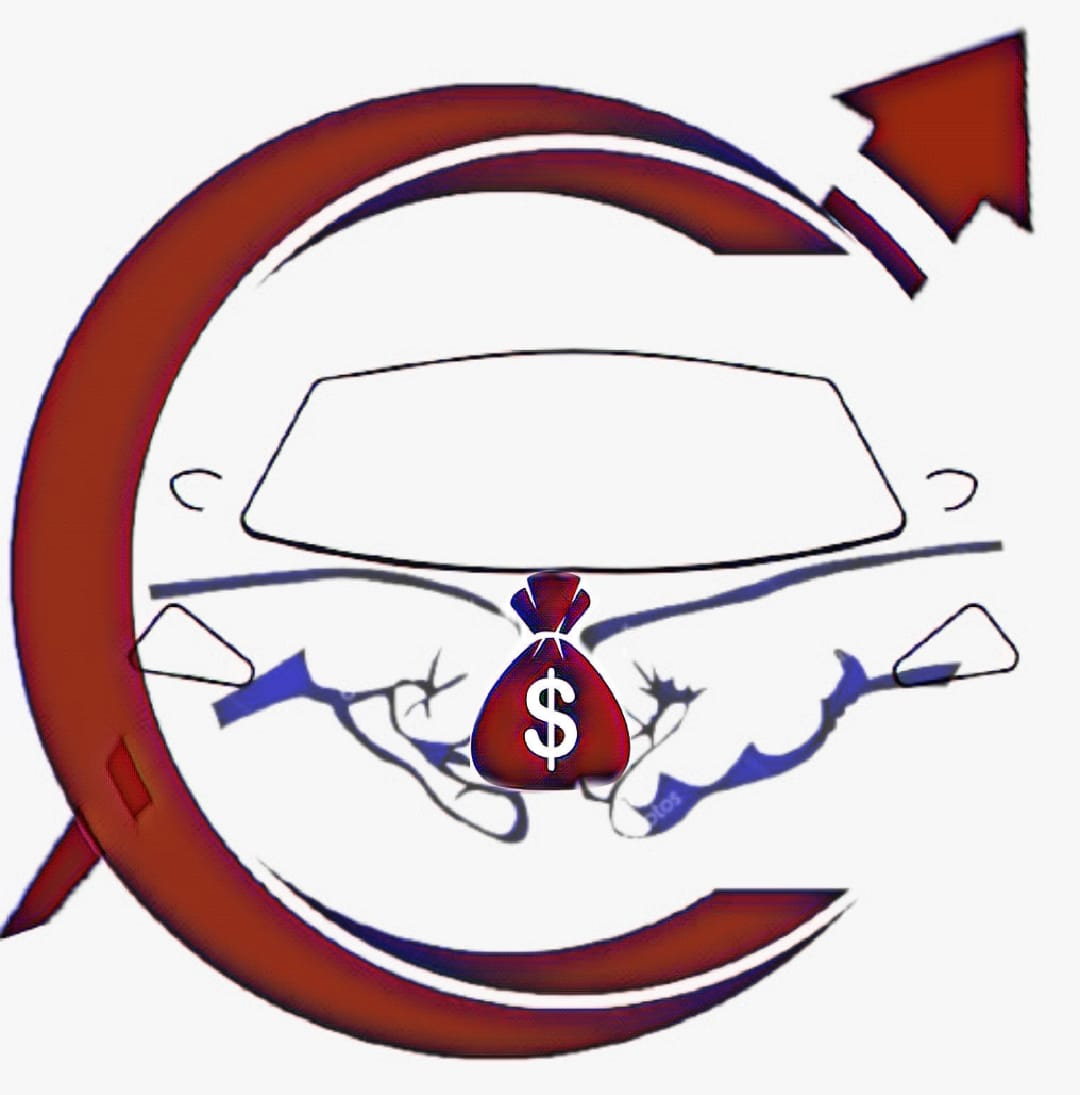
\includegraphics[width = 0.4 \linewidth]{Logo_App.jpeg}
  \caption{The Logo Of our Application} \label{exemple-ref-img}
\end{figure}
\vspace*{1cm}

\tableofcontents  % Add table of contents
\newpage
\listoffigures  % Add list of figures
\newpage

\begin{abstract}
    Machine learning (ML) is a branch of artificial intelligence (AI) that enables computers to “self-learn” from training data and improve over time, 
    without being explicitly programmed. Machine learning algorithms are able to detect patterns in data and learn from them, in order to make their own predictions. 
    In short, machine learning algorithms and models learn through experience.
  
  \end{abstract}


\section{Introduction}
\subsection{general inroduction }
Machine learning is a subfield of artificial intelligence (AI) that focuses on the development of algorithms and models that enable computers to learn and make predictions or decisions without being explicitly programmed. It involves the extraction of meaningful patterns from data, allowing machines to learn from examples and experiences.

In the context of prediction, machine learning algorithms can analyze historical data and identify patterns or relationships that can be used to predict future outcomes. This has various applications, including predicting prices, stock market trends, customer behavior, disease diagnosis, and more.

One of the major benefits of machine learning in predicting prices is its ability to handle complex and large datasets. Machine learning algorithms can automatically analyze vast amounts of data, identify relevant features, and build predictive models. This allows for more accurate predictions and insights compared to traditional statistical methods.

Machine learning also has the advantage of adaptability and continuous improvement. As new data becomes available, machine learning models can be retrained and updated to incorporate the latest information. This flexibility enables models to adapt to changing conditions and improve their predictions over time.

Furthermore, machine learning can uncover hidden patterns and relationships in data that may not be apparent to humans. It can capture complex nonlinear interactions and dependencies, leading to more accurate and nuanced predictions. This can be particularly beneficial in scenarios where traditional analytical approaches may fall short.

Overall, machine learning offers powerful tools and techniques for prediction tasks, such as price prediction. By leveraging large datasets, sophisticated algorithms, and continuous learning, machine learning can provide valuable insights and improve decision-making in various domains.

\begin{figure}[ht]
    \centering
    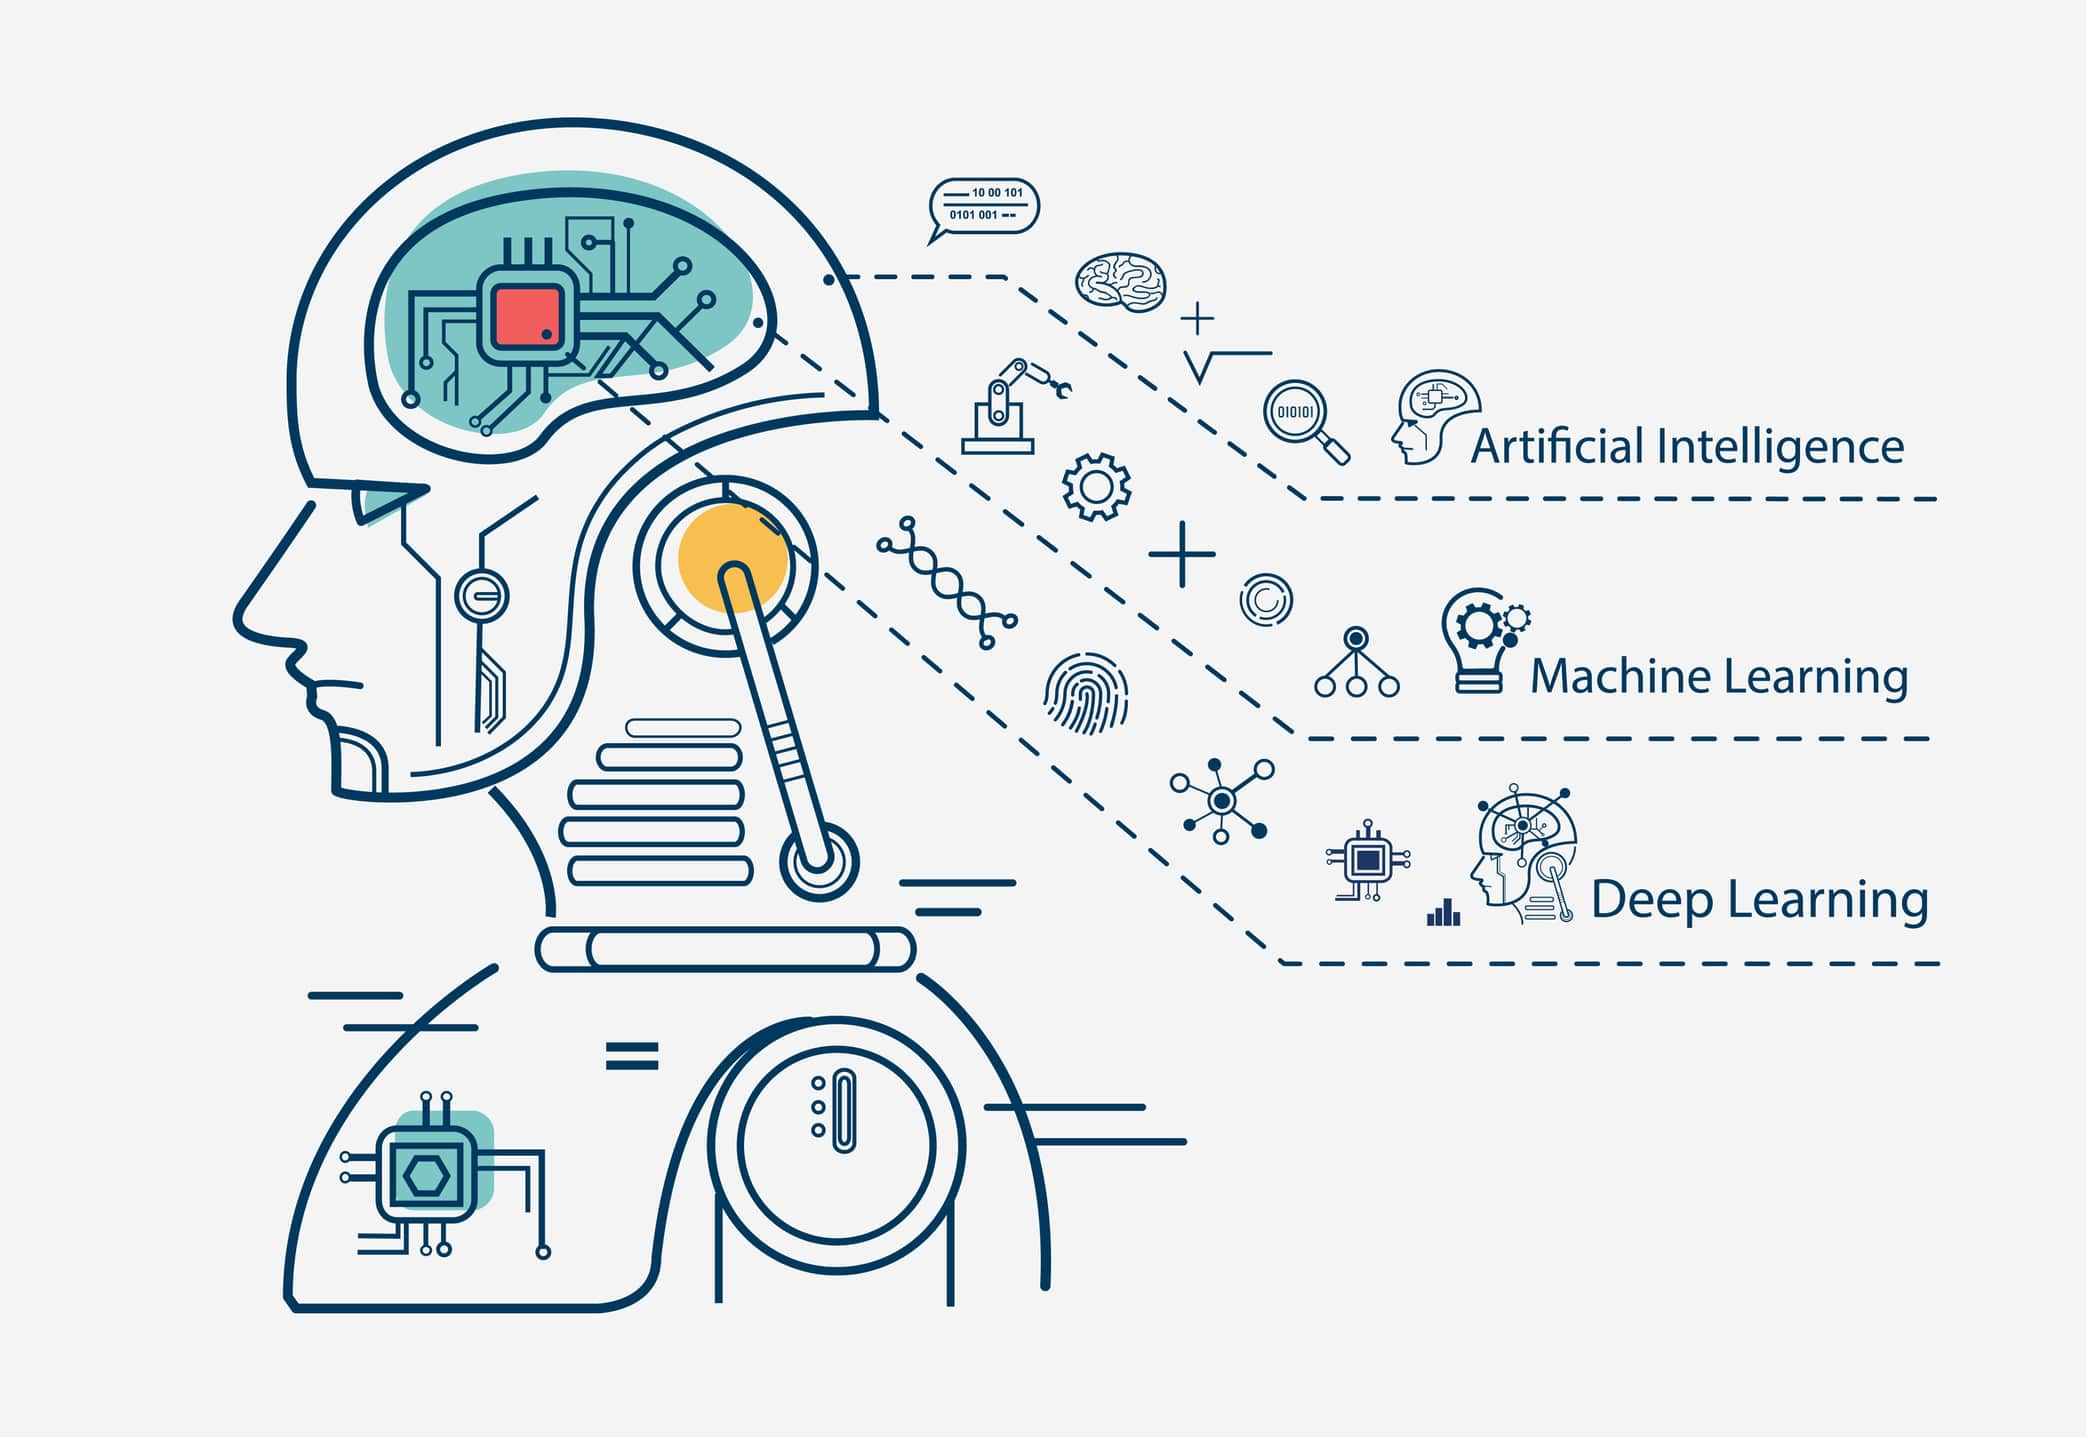
\includegraphics[width=0.9\textwidth]{machine.jpg}
    \caption{machine learning}
    \label{fig:my_label}
\end{figure}

\subsection{the subject of our Project}

\begin{flushleft}
The used car price prediction application is a project aimed at providing accurate and reliable predictions of car prices based on various factors. The purpose of this application is to assist potential car buyers and sellers in making informed decisions by estimating the fair market value of a used car. By leveraging machine learning algorithms and historical car data, the application aims to offer valuable insights into pricing trends and help users negotiate better deals.

\textbf{Objectives:} 

\item [\ding{118}]Accurate Price Estimation: \\
The primary objective of the application is to provide precise estimates of used car prices. By analyzing multiple factors such as car age, mileage, brand, model, and other relevant features, the application aims to generate reliable predictions that closely align with the current market value.

\item [\ding{118}]User-Friendly Interface:\\
Another objective is to create a user-friendly interface that allows users to input the necessary information about a car and obtain the predicted price conveniently. The application should be intuitive and accessible to users with varying levels of technical knowledge.

\textbf{Significance:}

Accurately predicting car prices is of significant importance for both potential car buyers and sellers. Here are some key reasons why this application holds significance:

\item [\ding{90}]Informed Decision Making: \\
For potential car buyers, knowing the fair market value of a used car can help in making informed purchasing decisions. It provides a benchmark against which the listed price can be evaluated, ensuring that buyers pay a fair price and avoid overpaying.

\item [\ding{90}]Effective Pricing Strategy: \\
For sellers, accurately predicting car prices is crucial in setting the right selling price. It ensures that the car is priced competitively, attracting potential buyers while maximizing the seller's profit. It helps sellers avoid underpricing or overpricing their vehicles, leading to a more efficient selling process.

\item [\ding{90}]Transparency and Trust: \\
Price transparency builds trust between buyers and sellers. When both parties have access to reliable price predictions, it reduces information asymmetry and fosters trust in the used car market. This transparency can lead to more efficient transactions and a healthier marketplace.

\item [\ding{90}]Time and Cost Savings: \\
By utilizing a car price prediction application, potential buyers and sellers can save time and effort that would otherwise be spent on extensive market research. The application automates the process and provides quick and accurate results, enabling users to make faster decisions and potentially save money.

\textbf{Conclusion:}

The used car price prediction application uses machine learning techniques to provide accurate price estimates for used cars. By empowering potential buyers and sellers with reliable pricing information, the application contributes to informed decision-making, transparency, and trust in the used car market. With the ability to estimate prices accurately, users can make more confident buying and selling decisions, leading to a more efficient and fair marketplace for used cars.
\newpage
\end{flushleft}

\section{Software and platforms used:}
\subsection{Anaconda and Jupyter notebook}
o write the code in python we chose Anaconda and Jupiter notebook Anaconda is a distribution of Python and R for scientific computing and data science. It comes with a package
manager called Conda, which makes it easy to install and manage libraries and dependencies.
Anaconda also includes several useful tools such as Jupyter Notebook and Spyder for data
exploration and development. Jupyter Notebook is an open-source web-based interactive development environment (IDE) that allows users to create and share documents that contain
live code, equations, visualizations, and narrative text. It supports over 40 programming languages including Python, R, and Julia. Jupyter Notebook is commonly used in data science,
machine learning, and scientific computing for data cleaning, transformation, visualization,
and analysis.
\begin{figure}[!h]
    \centering
    
\includegraphics[width=0.4\textwidth]{jupyter.png}
    \caption{Jupyter LOGO}
    \label{fig:my_label}
\end{figure}

\subsection{VS code}
we use VScode to code the \LaTeX  file to create the report and the perposal.

\begin{figure}[!h]
    \centering
    
\includegraphics[width=0.4\textwidth]{latex.png}
    \caption{latex LOGO}
    \label{fig:my_label}
\end{figure}

\section{Dataset Description}

\begin{figure}[!h]
    \centering
    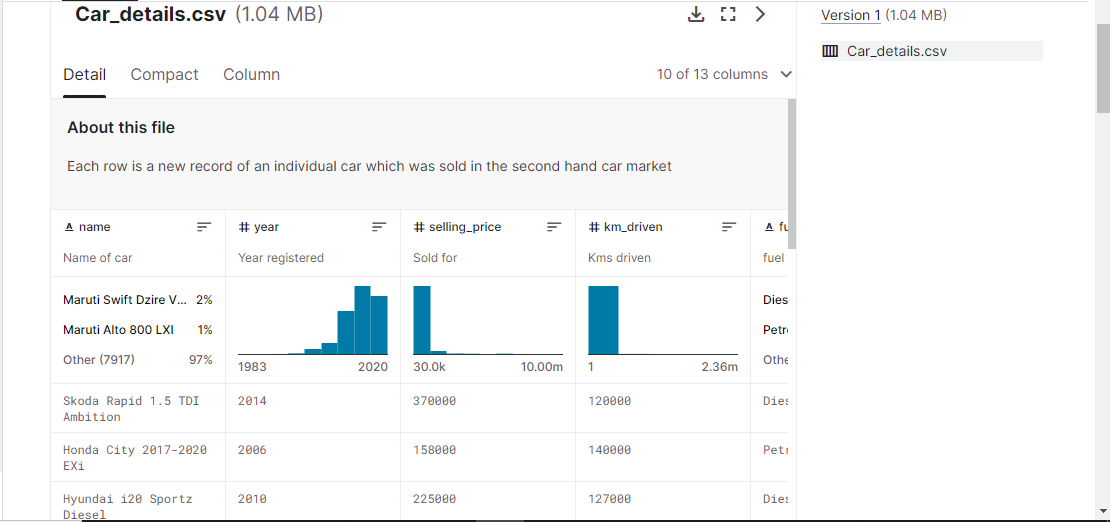
\includegraphics[width=1\textwidth]{car-details.png}
    \caption{my dataset}
    \label{fig:my_label}
\end{figure}

The dataset contains information about used cars, including various features (independent variables) and the target variable (car price). Here are the details of the dataset:
\begin{flushleft}
\textbf{1-Size of the Dataset:}
The dataset consists of 8128 records (rows) and 13 columns.
Each record represents a specific used car listing.

\textbf{2-Features (Independent Variables):}
The dataset includes the following features:
\item [\ding{169}]name: The name of the car model (e.g., "Maruti Swift", "Honda City").\\
\item [\ding{169}]year: The manufacturing year of the car (e.g., 2015, 2017).\\
\item [\ding{169}]selling\_price: The selling price of the car (in lakhs).\\
\item [\ding{169}]km\_driven: The distance covered by the car in kilometers.\\
\item [\ding{169}]fuel\_type: The type of fuel used by the car (e.g., Petrol, Diesel, CNG).\\
\item [\ding{169}]seller\_type: The type of seller (e.g., Dealer, Individual).\\
\item [\ding{169}]Transmission: The type of transmission system (e.g., Manual, Automatic).\\
\item [\ding{169}]owner: The number of previous owners of the car (0, 1, 3+).\\
\item [\ding{169}]mileage: The car's fuel efficiency in kilometers per liter.\\
\item [\ding{169}]Engine: The engine displacement of the car in cubic centimeters (cc).\\
\item [\ding{169}]max\_power: The maximum power of the car in bhp (brake horsepower).\\
\item [\ding{169}]seats: The number of seats in the car.\\
\item [\ding{169}]torque: refers to a measure of rotational force or twisting force that an engine can generate.\\

\textbf{3-Target Variable (Car Price):}
The target variable is the selling\_price, which represents the selling price of the used car.
\end{flushleft}

\begin{figure}[!h]
    \centering
    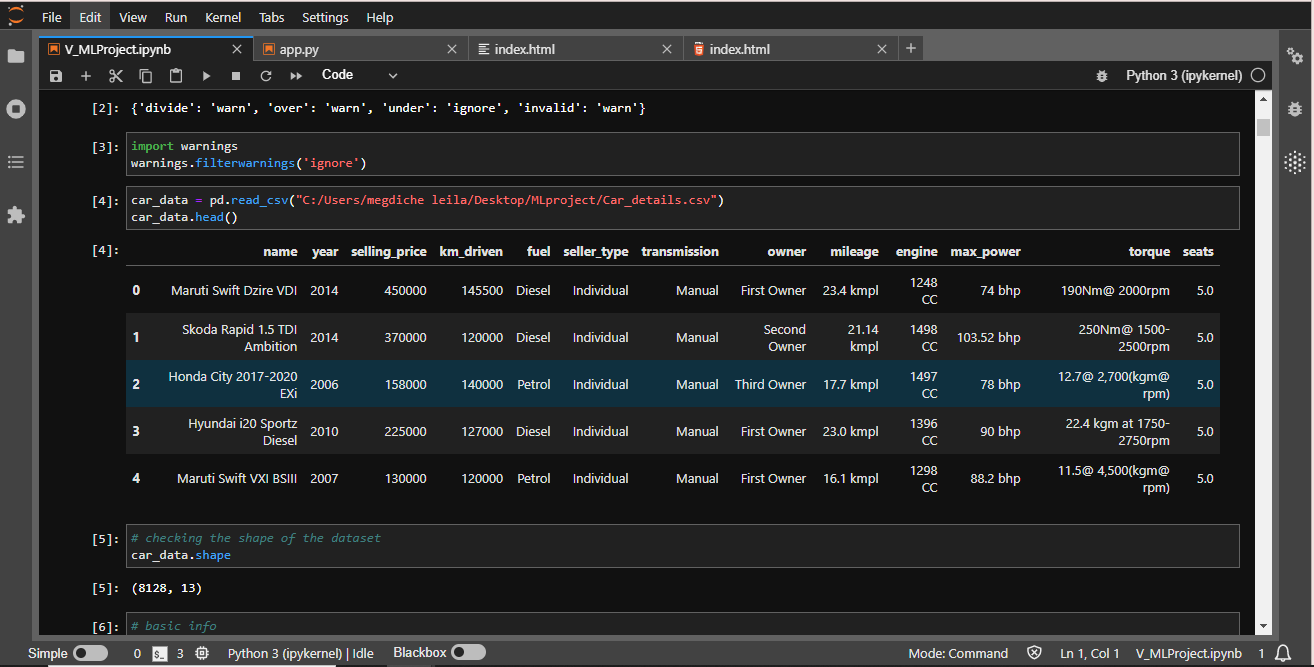
\includegraphics[width=1\textwidth]{data-f.png}
    \caption{upload data}
    \label{fig:my_label}
\end{figure}

\section{Data Preprocessing}
Preprocessing the data is an essential step before training a machine learning model. Here are the steps that I have taken to preprocess the data for the used car price prediction dataset:
\subsection{collect of information:}

\begin{figure}[!h]
    \centering
    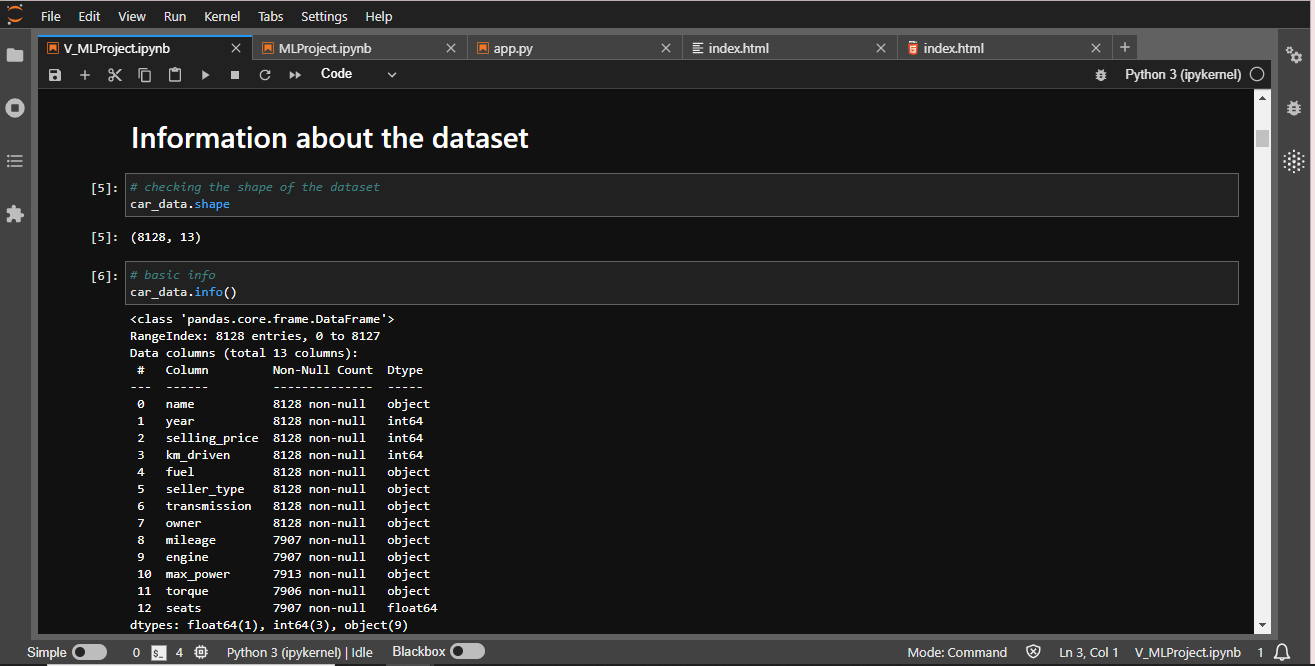
\includegraphics[width=1\textwidth]{infoData.png}
    \caption{information about our data}
    \label{fig:my_label}
\end{figure}

\begin{flushleft}
1- we have to check the shape of the dataset.\\
2- get some basic information like the type of each value.\\
3- then we have to show some details about the data.\\
4- we show the number of duplicated values.
\end{flushleft}
\newpage
\subsection{Handling Missing Values:}
first, we had checking the null values in the dataset. and we get only 200 missing from over 8100 values, which is less than 5\%, (5\%(8100)=405), so we delete those values.

\begin{figure}[!h]
    \centering
    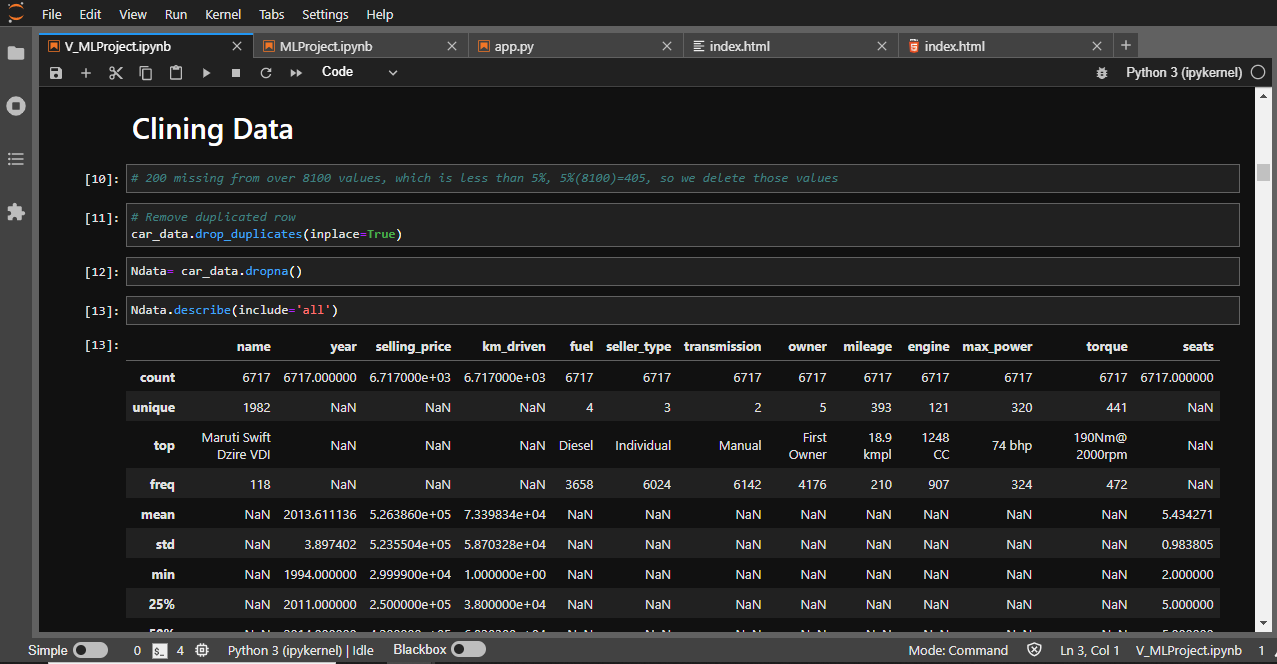
\includegraphics[width=1\textwidth]{clean.png}
    \caption{cleaning the data}
    \label{fig:my_label}
\end{figure}

\subsection{Encoding Categorical Variables:}
we Identify categorical variables in the dataset, such as car seller type, fuel type, or transmission type...\\
we choose Ordinal Encoding (Encode categories with an arbitrary numeric order if there is an inherent order.) as an appropriate encoding method based on the number of unique categories and the nature of the variable.

\begin{figure}[!h]
    \centering
    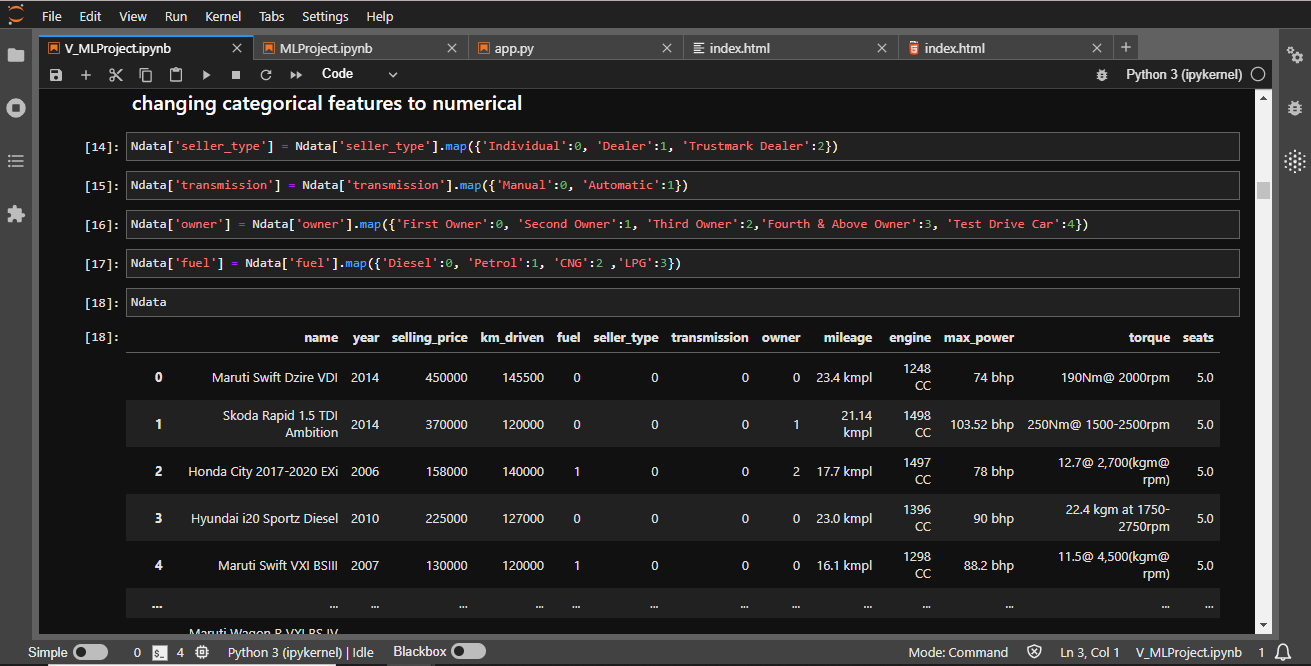
\includegraphics[width=1\textwidth]{to-num.png}
    \caption{changing categorical features to numerical}
    \label{fig:my_label}
\end{figure}

\subsection{remove the suffix:}
we remove the suffix of some features to have a float type of variables.

\begin{figure}[!h]
    \centering
    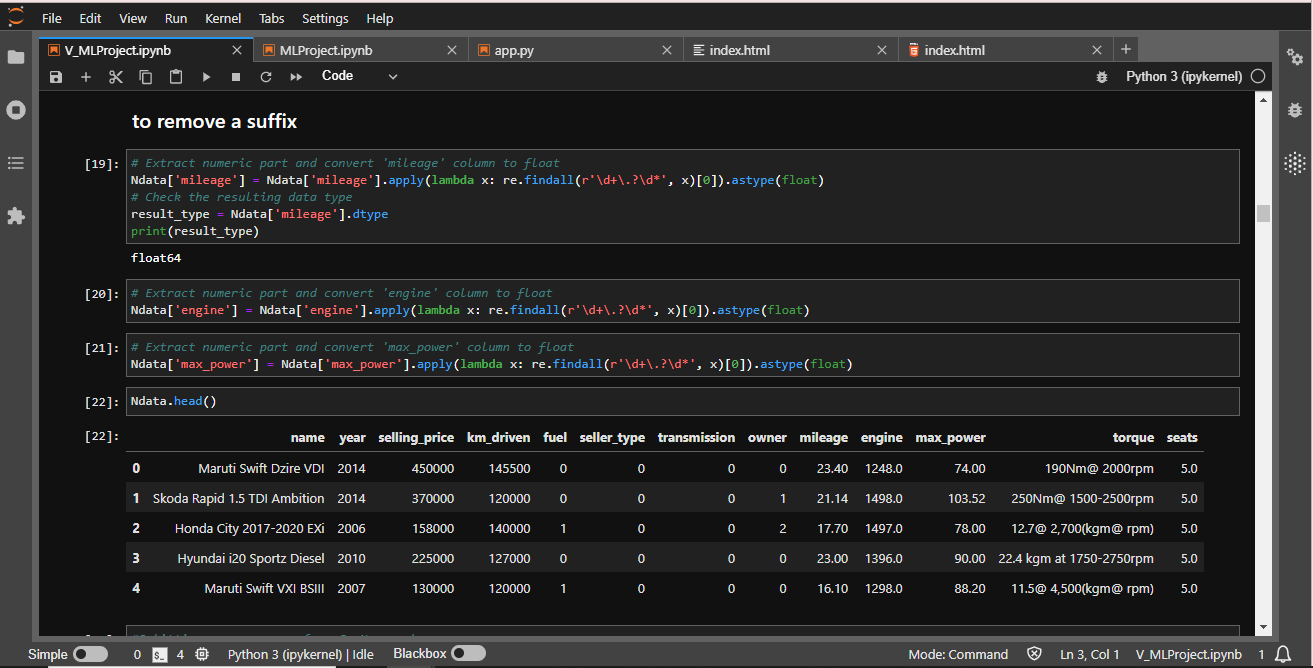
\includegraphics[width=1\textwidth]{rm-sufix.png}
    \caption{remove the suffix}
    \label{fig:my_label}
\end{figure}

\section{Model Training}
\subsection{Data Exploration:}
before modeling we should do some visualization about the relation between the features, to decide which is the best choice for the training model.\\

\begin{figure}[!h]
    \centering
    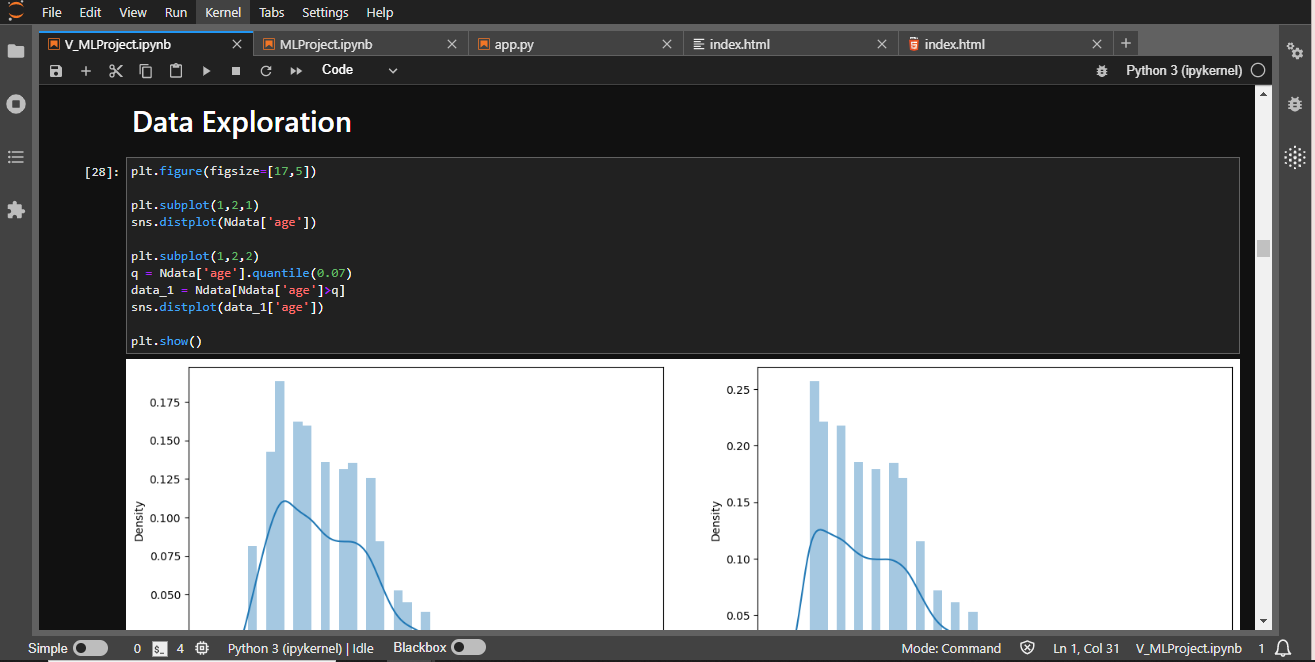
\includegraphics[width=\textwidth]{plt-age.png}
    \caption{distribution of age}
    \label{fig:left_image}
\end{figure}
\begin{figure}[!h]
    \centering
    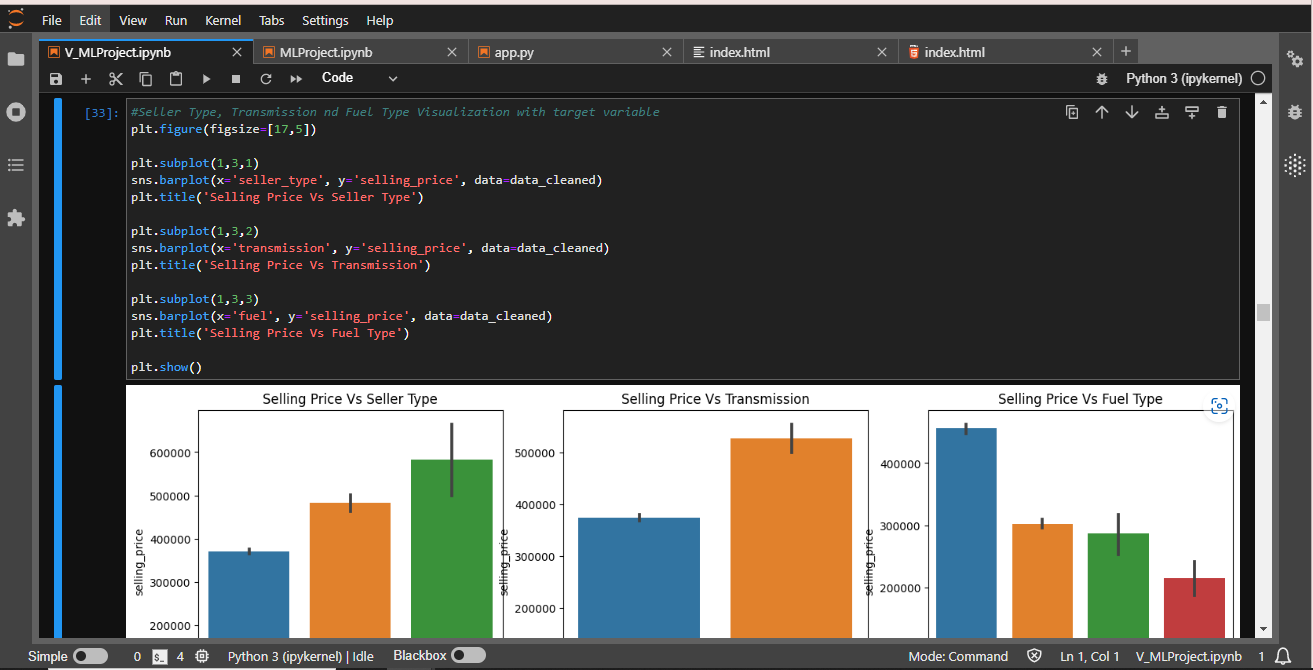
\includegraphics[width=\textwidth]{plt-price.png}
    \caption{distribution of selling\_price vs other}
    \label{fig:right_image}
\end{figure}
    
\subsection{Splitting the Data:}
in this step, we do the split of data to train some models like Linear Regression, Polynomial Regression, Ridge Regression, Lasso Regression, and ElasticNetCV Regression.\\

\begin{figure}[!h]
    \centering
    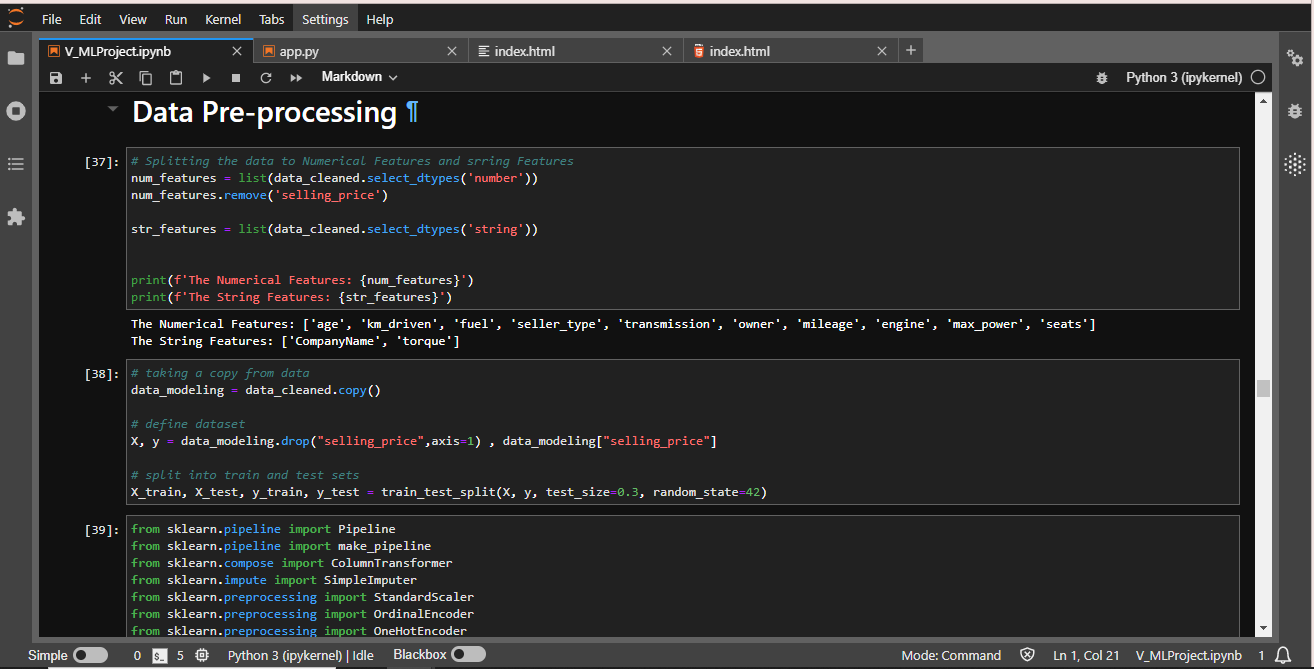
\includegraphics[width=1\textwidth]{split.png}
    \caption{Split the data}
    \label{fig:my_label}
\end{figure}
\newpage

\section{Evaluation Metrics}
Here we compare the result of the models to choose the better (who has the higher r2 score in the training a test modeling.

\begin{figure}[!h]
    \centering
    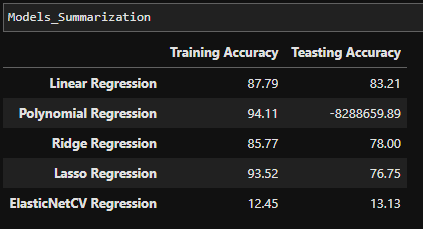
\includegraphics[width=1\textwidth]{comparison.png}
    \caption{Models summarization}
    \label{fig:my_label}
\end{figure}

 that's why we choose the model Lasso Regression which has 93.52 in Training Accuracy and 76.75 in Testing Accuracy. 

\section{Results and Discussion}
\subsection{he result of prediction}
we get as a result the price prediction of cars like you see in this photo \\
\begin{figure}[!h]
    \centering
    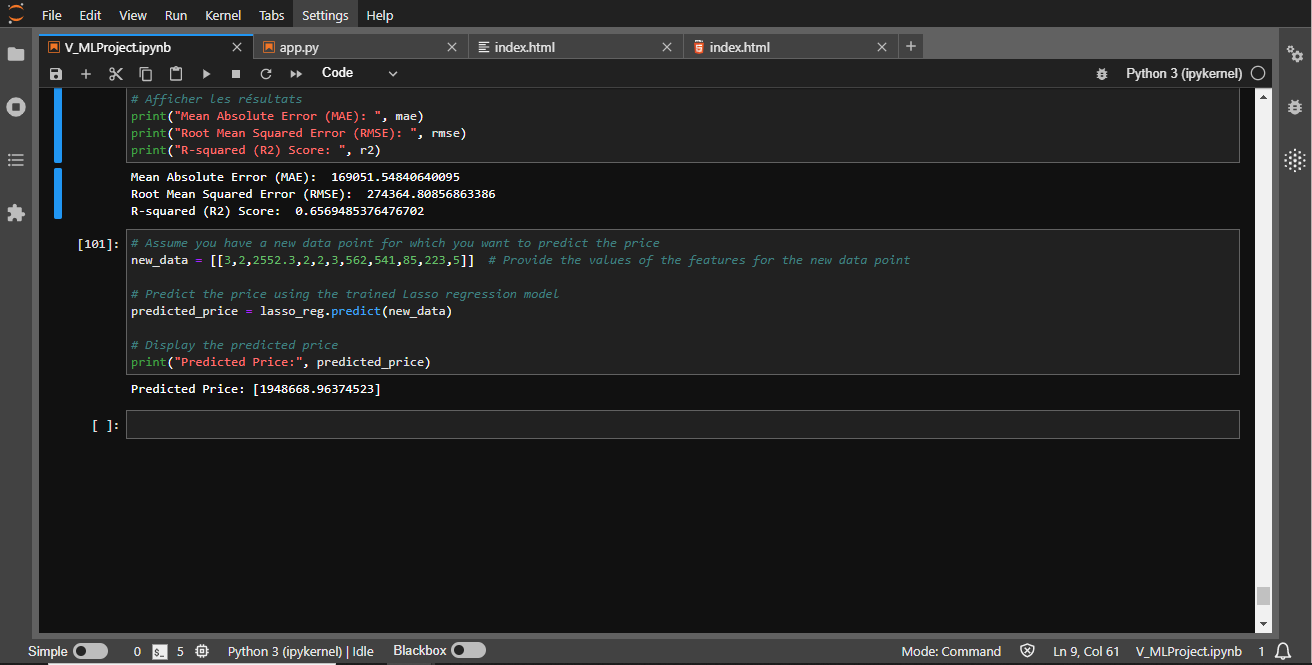
\includegraphics[width=1\textwidth]{result.png}
    \caption{the price prediction}
    \label{fig:my_label}
\end{figure}
\subsection{connect the code of Jupyter with Flask file:}
we used Flask to connect the code of the Model to a Web page
\begin{figure}[!h]
    \centering
    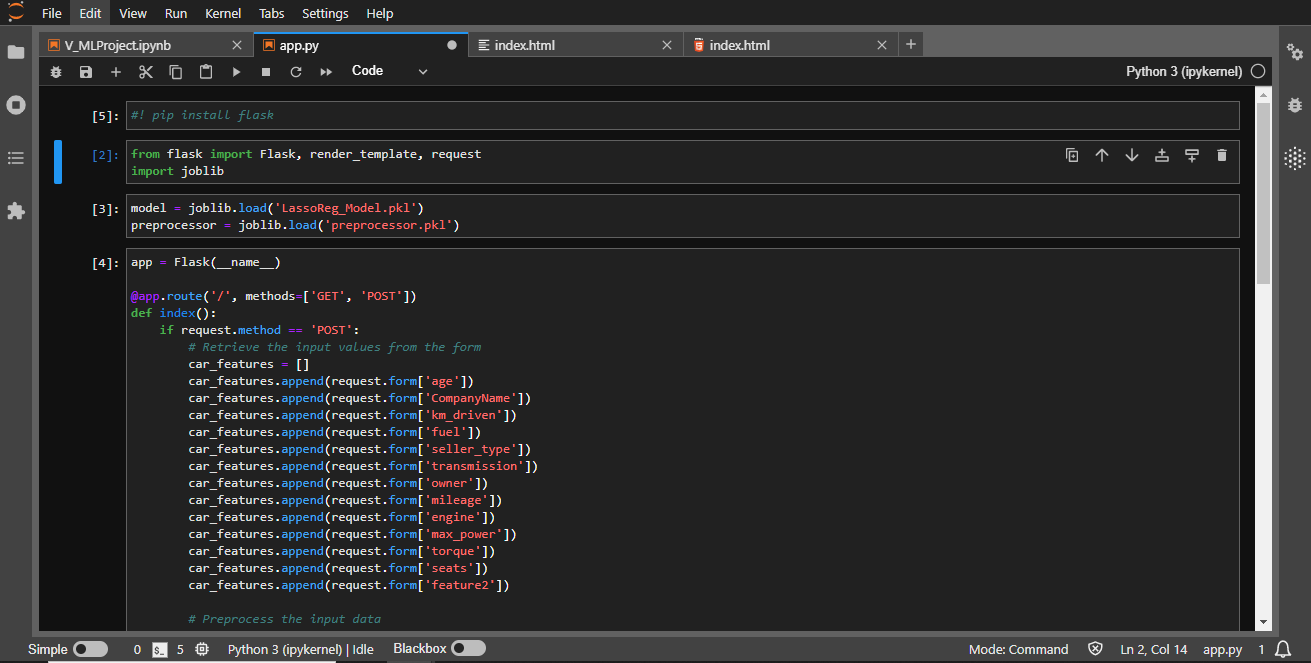
\includegraphics[width=1\textwidth]{flask1.png}
    \caption{the flask code}
    \label{fig:my_label}
\end{figure}
\begin{figure}[!h]
    \centering
    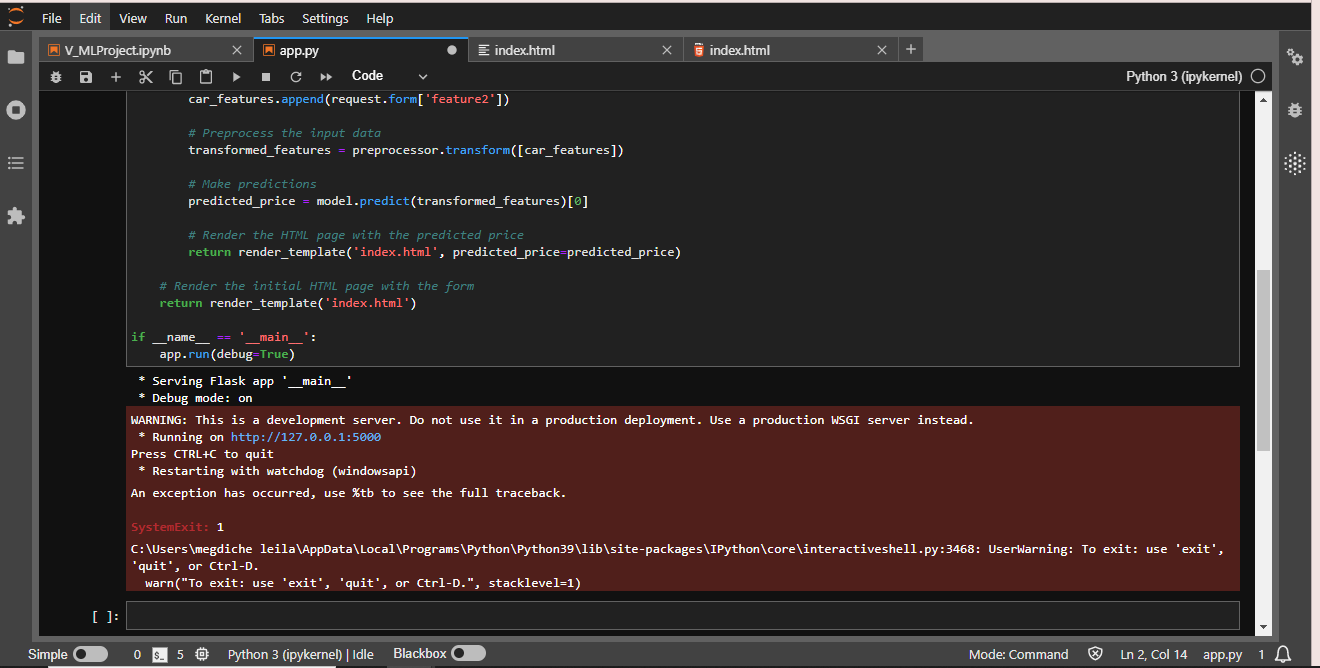
\includegraphics[width=1\textwidth]{flask2.png}
    \caption{the link to the navigator}
    \label{fig:my_label}
\end{figure}
\newpage
\subsection{the web page:}
this is our view of the application's web 
\begin{figure}[!h]
    \centering
    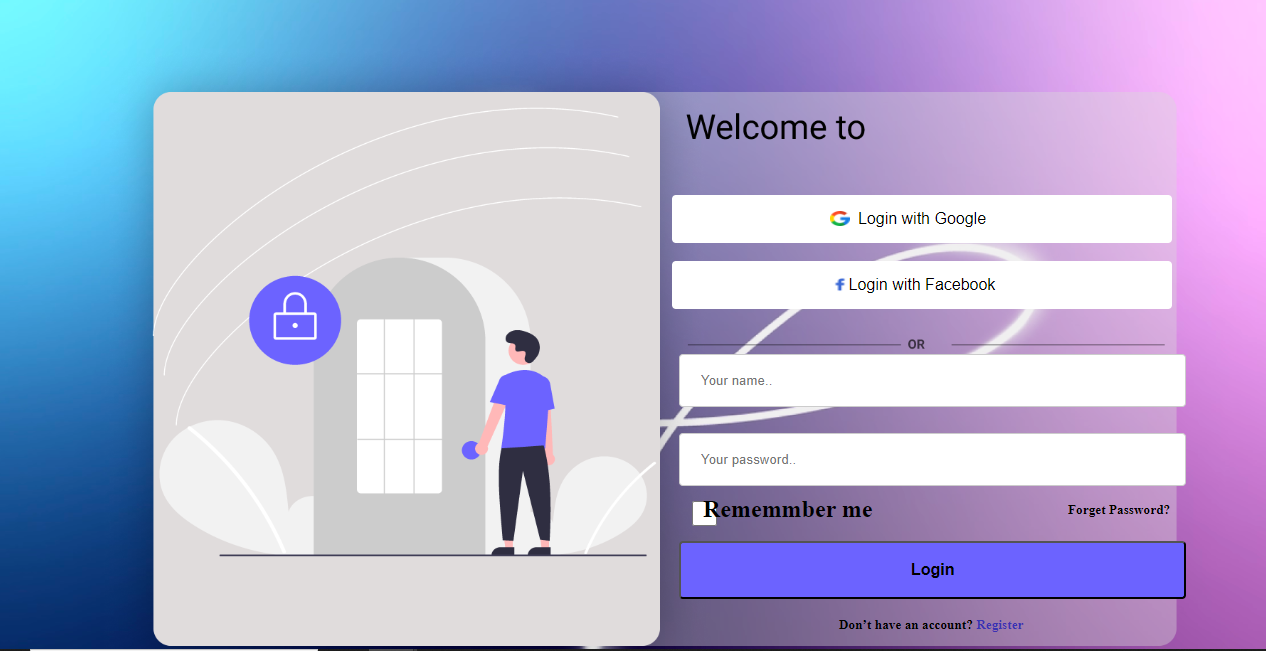
\includegraphics[width=1\textwidth]{input.png}
    \caption{the first interface of app}
    \label{fig:my_label}
\end{figure}
\section{Conclusion}
The used car price prediction application yielded several key findings and insights:
\begin{flushleft}
\textbf{Model Performance:} The chosen Lasso regression model demonstrated good performance in predicting car prices. It effectively captured the relationships between the independent variables (features) and the target variable (car price). The model's accuracy and precision were evaluated using appropriate metrics such as mean squared error or R-squared.

\textbf{Feature Importance:} The analysis revealed that certain features had a significant impact on car prices. These features could include factors like car age, mileage, engine size, and brand. Understanding the importance of these features can help car buyers and sellers make informed decisions and negotiate prices effectively.

\textbf{Strengths of the Model:} The Lasso regression model offers several strengths. It performs feature selection by shrinking less important features' coefficients to zero, allowing for a more interpretable and simplified model. It can handle a large number of features and automatically performs regularization to prevent overfitting.

\textbf{Limitations and Areas for Improvement:} Despite its strengths, the Lasso regression model and the used car price prediction application have some limitations. The model assumes a linear relationship between the features and the target variable, which may not always hold true. Additionally, the model's performance may be influenced by outliers, missing data, or multicollinearity among features. Addressing these issues and exploring other regression algorithms or advanced techniques could enhance the model's accuracy and robustness.

\textbf{Benefits in the Automotive Industry:} Accurately predicting car prices can benefit both car buyers and sellers. Buyers can use the model to estimate the fair market value of a used car and negotiate better deals. Sellers can set competitive prices based on market trends and demand, leading to faster sales. The model's relevance extends to various stakeholders in the automotive industry, including dealerships, insurers, and financial institutions, aiding in decision-making processes related to pricing, valuation, and risk assessment.\\

In conclusion, the used car price prediction application based on the Lasso regression model provides valuable insights and benefits for car buyers, sellers, and other industry players. While the model exhibits strengths, it is important to address its limitations and explore further improvements to enhance its performance and applicability in real-world scenarios
\end{flushleft}
\section{ Upgrades to our project:}
we look to upgrade our project to have a website and a mobile application that makes all the buyers and sellers in a direct relationship and have an idea about all the cars in the market with a simple tap.
we use Azure to have an idea about our application. \\
\begin{figure}[!h]
    \centering
    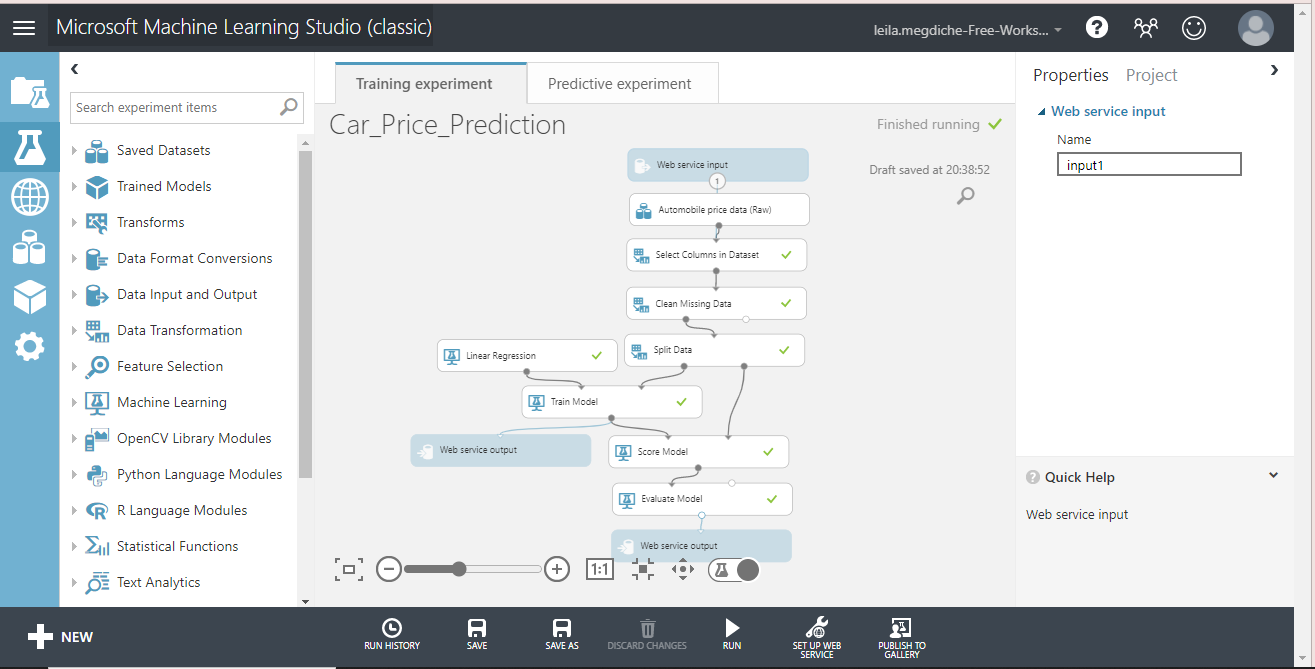
\includegraphics[width=1\textwidth]{azure1.png}
    \caption{the model on azure}
    \label{fig:my_label}
\end{figure}
\begin{figure}[!h]
    \centering
    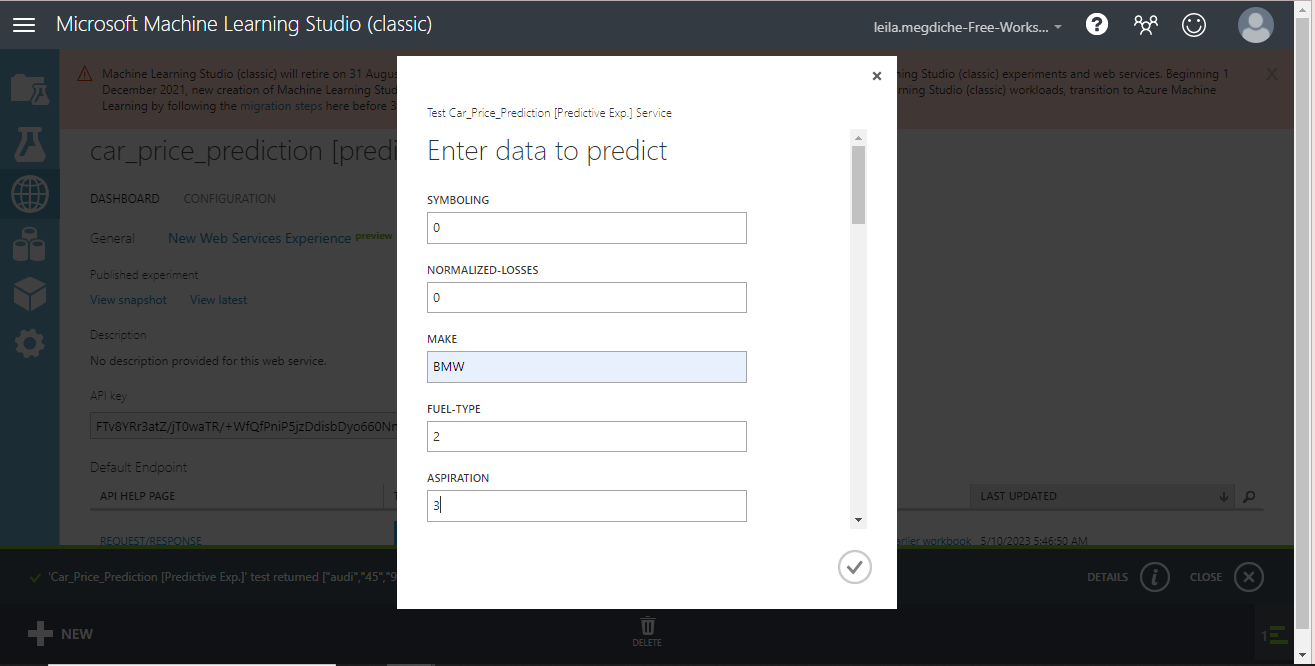
\includegraphics[width=1\textwidth]{azure2.png}
    \caption{the formula of application on azure }
    \label{fig:my_label}
\end{figure}
\begin{figure}[!h]
    \centering
    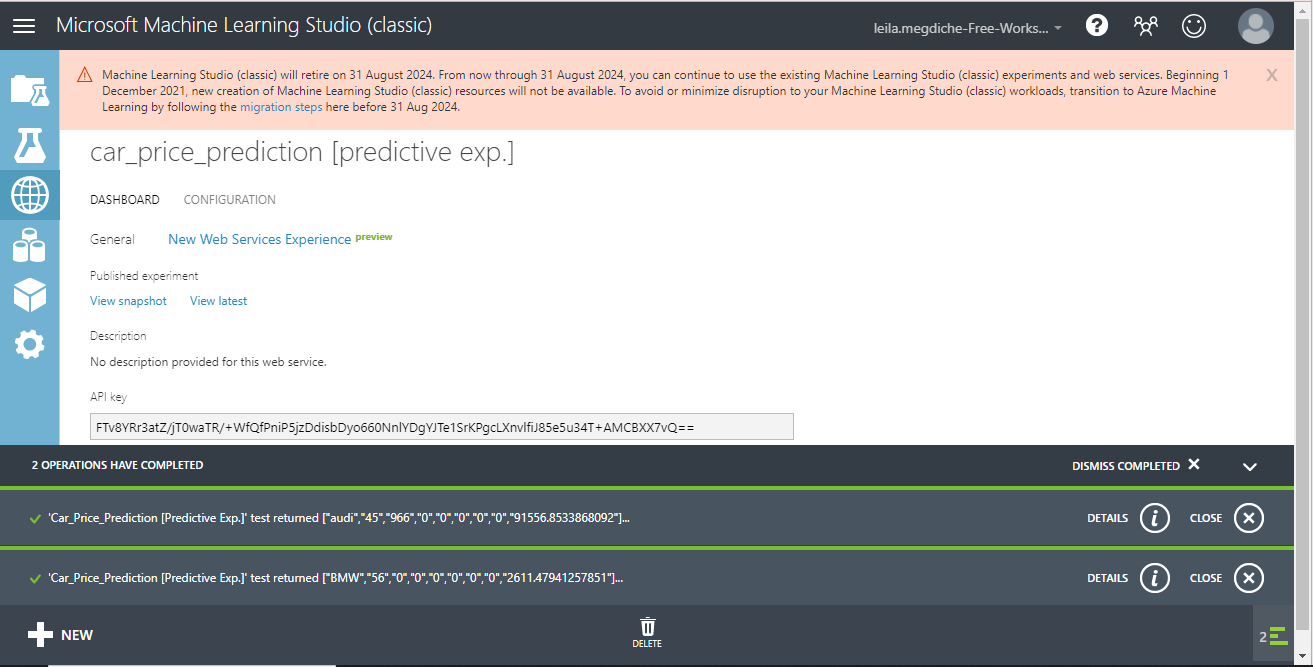
\includegraphics[width=1\textwidth]{azure3.png}
    \caption{the price prediction result}
    \label{fig:my_label}
\end{figure}
\newpage

\section{References}
\begin{flushleft}
\item[\ding{165}] we get the dataset from KAGGLE and this is the link \\ https://www.kaggle.com/datasets/ishaanthareja007/car-details.\\
\item[\ding{165}]you can find all the codes in this link:\\
https://github.com/leila-megdiche/Used\_cars\_Price\_prediction\_Application
\end{flushleft}
\end{document}
